
\documentclass[12pt]{article}

\usepackage{amssymb}
\usepackage{amsmath}
\usepackage{amsthm}
\usepackage{amsfonts}
\usepackage{enumitem}
\usepackage{graphicx}
\usepackage{float}
\usepackage[margin=1in]{geometry}

\newenvironment{solution}
  {\par\noindent\textbf{Solution:}\par}
  {\par}
\title{MATH 340, 2024/25, Term 2, Assignment 1}
\author{Mercury Mcindoe 85594505} 

\begin{document}
\maketitle 
\thispagestyle{empty}
  
\begin{enumerate}
  \item Essay

    \pagebreak

\item You should study the self-study material on the standard forms of LP, available in the Canvas/Files. Put the following linear programming problem in standard form, that is, standard inequality form. (Do not solve)
    \begin{align*}
    &\text{minimize } && x_1 - 3x_2 \\
    &\text{subject to } && x_1 + x_2 = 2 \\
    & && x_1 \ge 3 \\
    & && x_2 \text{ unconstrained}
\end{align*}

\begin{solution}
  Let's start with transforming the constaints to standard form,
  $$x_1 \ge 3 \to x_1 - 3 \ge 0, \text{ and let } x_1' = x_1 - 3$$
  $$x_2 \text{ unconstrained} \to x_2 = x_2^+ - x_2^-, \hspace{.05in} x_2^+, x_2^- \ge 0$$
  $$x_1 + x_2 = 2 \to x_1 + x_2 \le 2,\hspace{.05in} -x_1 - x_2 \le -2 $$
\end{solution}

Now, let's change the constraints with respect to $x_1',x_2^+,x_2^-$,
$$x_1' + 3 + x_2^+ - x_2^- \le 2 \to x_1' + x_2^+  - x_2^- \le -1$$
$$-(x_1' +3) -(x_2^+ - x_2^-) \le -2 \to -x_1' -x_2^+ + x_2^- \le 1 $$
$$x_1 \ge 3, \hspace{.05in} x_2 \text{ unconstrained} \to x_1' , x_2^+,xv_2^- \ge 0 \text{ where } x_1' = x_1-3,x_2 = x_2^+ -x_2^-$$

The objective function is then,
$$\text{min}(x_1-3x_2) \to -\text{max}(-x_1+3x_2) = -\text{max}(-x_1'-3 + 3x_2^+ -3x_2^-)$$
$$\to 3 - \text{max}(-x_1'+3x_2^+-3x_2^-)$$
Hence,
\begin{align*}
 &\text{maximize } && -x_1'+3x_2^+-3x_2^- \\
    &\text{subject to } && x_1' + x_2^+ - x_2^- \le -1 \\
    & && -x_1'-x_2^+ + x_2^- \le 1 \\
    & && x_1', x_2^+, x_2^- \ge 0 
\end{align*}


\item Consider a finite set of nonzero vectors, $v_1,v_2,\dots,v_k \in \mathbf{R}^n$, with $\left|v_i\right| > 0, i = 1, \dots, k;
  k \ge 1$. Define $$ C = \bigcap_{i=1}^k H_{v_i}$$ where we denote $$H_v = \{ x \in \mathbf{R}^n \hspace{.05in}\vert \hspace{.05in} v \cdot x \le 1 \}$$
 \begin{enumerate}[label=\alph*.] % Use a., b., c., ... format
   \item For the set $C$ defined in the above equation (1), is it possible for some case that $C=\emptyset$? Here, $\emptyset$ denotes the empty set. Justify you answer, either by giving such a case or proving that it is not possible.
   \begin{solution}
     No matter what finite set of vectors we have, each $H_v$ for some $v \in \mathbb{R}^n$ within that finite set of vectors 
     we would always have the zero vector $\textbf{0}$ included among that set. This is because we are interested 
     in the set of vectors such that $ v \cdot x \le 1$ is satisfied and for $ x = \textbf{0}$,

     $$v \cdot x = v \cdot \textbf{0} = 0 \le 1$$
     Hence, $\textbf{0} \in C$ in all cases.
  \end{solution}

   \item Give an example of the vectors $v_i \in \mathbf{R}^2$, with $\vert v_i \vert  > 0, i= 1,2,3,$ (so $n=2$ and $k=3$),where the set $C$ defined in the above equation (1), is a bounded set. Justify your answer clearly. \\ (Here, a set $S$ is said to be bounded, if there exists a positive number $K$ such that $\vert x \vert \le K$ for any $x \in S$. In other words, $S$ is bounded if it is contained in a ball (centred at the origin) of certain radius $K$.)
  \begin{solution}
    Let $v_1,v_2,v_3 \in \mathbf{R}^2$, where $v_1= \begin{bmatrix} 1 \\ 1\end{bmatrix}, v_2 = \begin{bmatrix} -1 \\ 0 \end{bmatrix} , v_3 = \begin{bmatrix} 0 \\ -1 \end{bmatrix}$. Also, let $x = \begin{bmatrix} x_1 \\ x_2 \end{bmatrix} \in \mathbf{R}^2$ where $x_1,x_2 \in \mathbb{R}$.\\ Then,
    $$H_{v_1} = \{ x \in \mathbf{R}^2 \hspace{.05in} \vert \hspace{.05in} x_1 + x_2 \le 1 \} $$
    $$H_{v_2} = \{ x \in \mathbf{R}^2 \hspace{.05in} \vert \hspace{.05in} -x_1\le 1 \} $$
$$H_{v_3} = \{ x \in \mathbf{R}^2 \hspace{.05in} \vert \hspace{.05in}  -x_2 \le 1 \} $$
If we plot the region corresponding to each $H_{v_i}$ the overlapping region ($C$) is highlighted as the following,
  \\  
\begin{figure}[H]
\centering
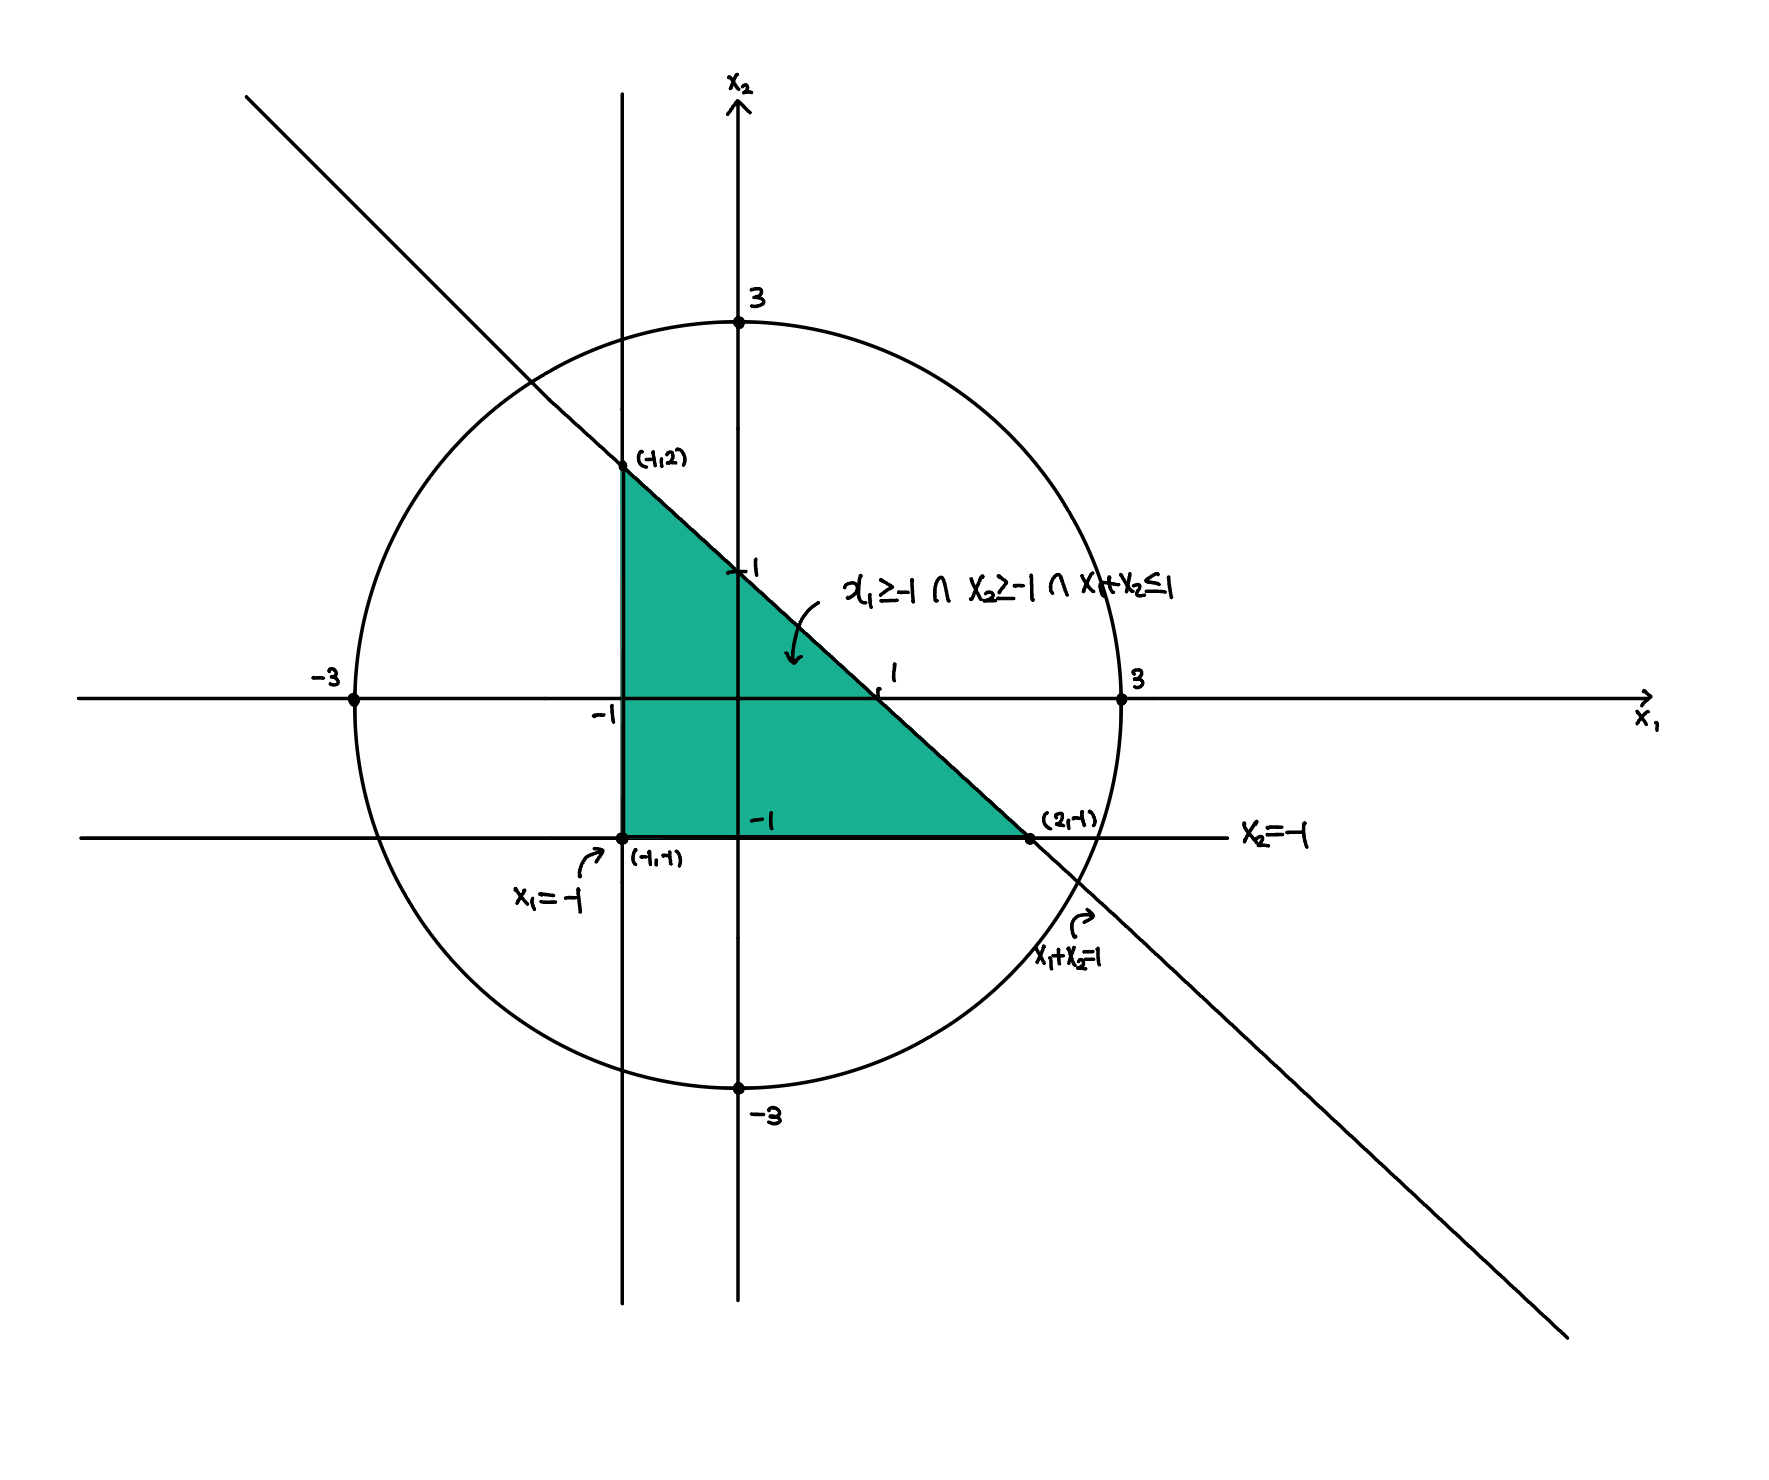
\includegraphics[width=0.6\textwidth]{figure1.jpg} 

\end{figure}

Which is can be contained in a ball of radius $3$ for instance, as shown in the figure, hence it is bounded.
\end{solution}

 \end{enumerate}

\item For a given $r > 0$, define $B_r \{ x \in \mathbf{R}^n \hspace{.05in} \vert \hspace{.05in} \vert x \vert \le r \}$, the ball of radius $r$ centered at the origin.
  \begin{enumerate}[label=\alph*.]
    \item Express $B_r$ as the intersection of \textbf{infinite} number of half spaces.
      \begin{solution}
        For $\mathbf{R}^n$, we can represent a ball of radius $r$ ($B_r$) centered at the origin as the following,
        $$x_1^2+x_2^2 + \cdots +x_n^2 = r^2$$
        where $x_1,\cdots,x_n \in \mathbb{R}$ and $x = \begin{bmatrix} x_1 \\ x_2 \\ \vdots \\ x_n \end{bmatrix} \in \mathbf{R}^n$.
        For a point on the surface of the ball $B_r$, say $a_1 = (a_{11},a_{12},\cdots,a_{1n}) \in \mathbb{R}^n$, the plane tangent to the ball $B_r$ would be 
        $$a_{11}x_1 + a_{12}x_2 + \cdots + a_{1n}x_n = r^2$$

        If we define $H_1$ as the halfspace $\{x \in \mathbf{R}^n \hspace{.05in} \vert \hspace{.05in} a_1 \cdot x \le r^2 \}$ we can contain the ball $B_r$ within that halfspace.
        \\ 
        Since there are infinitely many points on the surface of the ball $B_r$, we can create a halfspace in the same manner for each surface point like we constructed for $H_1$.
        Hence,
        $$B_r = \bigcap_{i \in S} H_i$$
        where $S$ is the set of surface points of $B_r$. And this is a intersection of an infinite number of halfspaces since there are infinitely many points on the surface of the ball.
  
      \end{solution}
    \item Can one express $B_r$ as the intersection of \textbf{finite} number of half spaces? Explain your answer in the two dimensional $\mathbf{R}^2$ case, by drawing relevant figures. (Your answer for this problem does not have to be rigorous. For example, a convincing figure and explanation of it would be sufficient.)
      \begin{solution}
        In contrast, let's assume that $B_r$ can be expressed as the intersection of finite number of half spaces. In order to have the ball represented as the intersection of these half spaces,
        one would need to create a halfspace per every point on the surface of $B_r$ which satisfies $\{ x \in \mathbb{R}^n \hspace{.05in} \vert \hspace{.05in} a \cdot x \le r^2 \}$ for a point on the surface called $a$.
        Then due to the assumption we made, it shows that $B_r$ is a polygon. Which contradicts with the fact that a ball is not a polytope, hence we cannot express $B_r$ as the intersection of finite number of halfspaces.
         \begin{figure}[H]
        \centering
        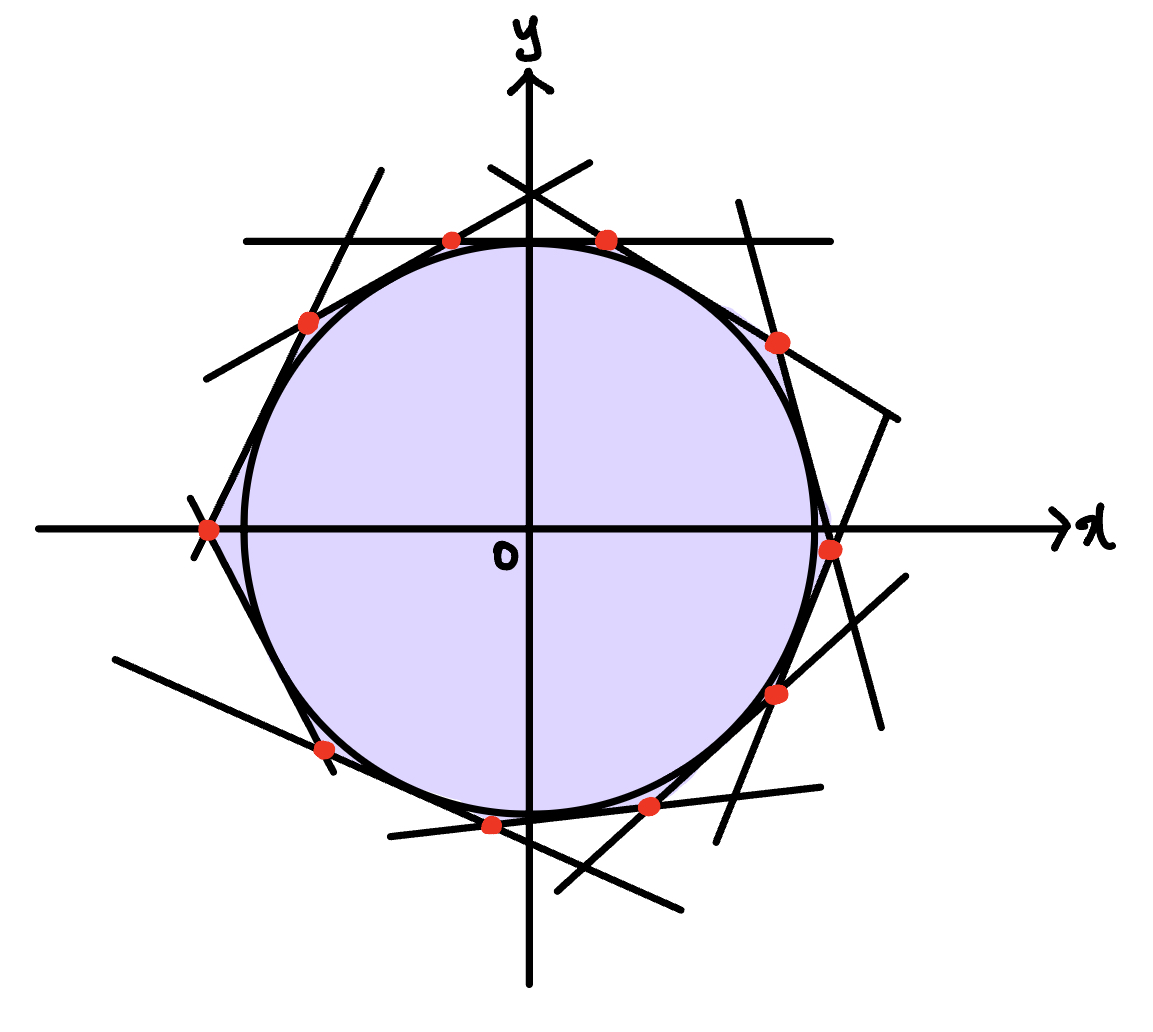
\includegraphics[width=0.5\textwidth]{figure3.jpg} 
      \end{figure}

      \end{solution}
  \end{enumerate}

  \pagebreak
\item Let $c$ be a given nonzero constant vector $c \neq 0 \in \mathbf{R}^n$. Let $r > 0$ be a given positive
  constant, and $B_r$, is the ball of radius $r$ centred at the origin: $B_r = \{x \in \mathbf{R}^n \hspace{.05in} \vert \hspace{.05in} x\le r\} $.
  Consider the following optimization problem:
    \begin{align*}
        &\text{(Prob)} && \text{Maximize }  c \cdot x \\
        & && \text{under the constraint: } x \in B_r.
    \end{align*}
    \begin{enumerate}[label=\alph*.]
      \item Express the optimal solution $\bar{x}$ of (Prob) in terms of $c$ and $r$. \\ (Hint: recalll the Cauchy-Schwarz inequality: $$c \cdot x \le \vert c \vert \vert x \vert$$ where the equality holds when and only when $c$ and $x$ are parallel, that is, $x=tc$ for some scalar $t >0 $.)
        \begin{solution}
          $c \cdot x$ would reach its maximum $\| c \|\cdot \| x \|$ only when $c$ and $x$ are parallel and are in the same direction, hence $c \cdot x > 0$. And this can only be satisfied when $x$ is parallel to $c$ with length $r$.

          $$\bar{x} = \frac{c}{\| c \|} \cdot r$$
        \end{solution}
      \item Draw an illustration (a picture) that explains this in the two dimensional case $(n=2.)$
           \begin{figure}[H]
        \centering
        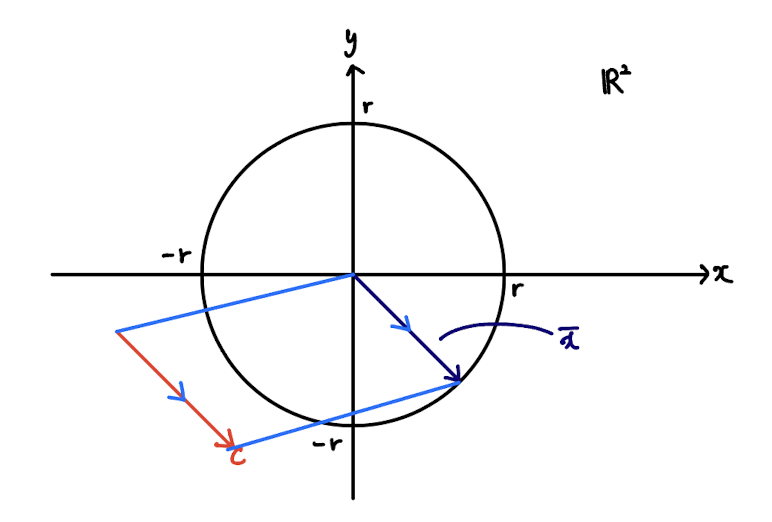
\includegraphics[width=0.5\textwidth]{figure2.png} 
      \end{figure}

    \end{enumerate}

  \item Let $C \subset \mathbf{R}^n$ be a given set and $C=\emptyset$. Let $f:\mathbf{R}^n \to \mathbf{R}$ be a given function. \\ Consider the following optimization problem:
    \begin{align*}
        &\text{(Prob1)} && \text{Maximize }  f(x) \\
        & && \text{under the constraint: } x \in C.
    \end{align*}
    For each real number $r \in \mathbf{R}$, define $F_r := \{ x \in \mathbf{R}^n \hspace{.05in} \vert \hspace{.05in} f(x) \ge r\}$, and consider 
    \begin{align*}
        &\text{(Prob2)} && \text{Maximize }  r \\
        & && \text{under the constraint: } C \cap F_r \neq \emptyset.
    \end{align*}
    Here the constraint $C \cap F_r \neq \emptyset$ is a condition on $r$. \\ 
    Assume that an optimal solution of (Prob1) and an optimal solution of (Prob2) both exist. 

    \begin{enumerate}[label=\alph*]
      \item Is it possible to have more than one optimal solution $\bar{r}$ of (Prob2)? Justify your answer. (Hint: What is the decision variable and the objective function of (Prob2)?)
        \begin{solution}
          Our goal is to maximize the object function $r$ while $C \cap F_r \neq \emptyset$. Let this maximized $r$ be $r_\text{max}$ while $C \cap F_r \neq \emptyset$. 
          Now assume to the contrary that there is another $r'$ such that $r' \neq r_\text{max}$ and $C \cap F_r \neq \emptyset$ for such $r'$, while $r$ is maximized.
          If $r' \neq r_\text{max}$, then either $r' > r_\text{max}$ or $r' < r_\text{max}$, in either case only one option can be chosen since the goal of the linear programming problem is to maximize $r$.
          Hence, we cannot have more than one optimal solution $\bar{r}$ of (Prob2).

        \end{solution}

      \item Find and explain the relation between the optimal solution of (Prob1) and that of (Prob2). You have to justify your answer. [Hint: To get an intuition, try first $n=1$ case and $n=2$ case, with a linear function $f$ and the set $C$ given by the linear constraints. Your final answer should be for general $n$ and for general $f$ and $C$.] [\textbf{This problem will be marked strictly: To get a nontrivial mark, please make your explanation very clear in a logical manner.}]
      % \begin{solution}
      % Let's call the optimal solution of (Prob1), $\bar{x}$ and (Prob2), $\bar{r}$. That means $\forall x \in C, f(x) \le f(\bar{x})$ and $\bar{r}$ is the largest $r$ we can achieve while maintaining $C \cap F_{\bar{r}} \neq \emptyset$. 
      % Let's consider the case where $\bar{x} \notin F_\bar{r}$, this means that $\exists x^* \in C \setminus (C \cap F_{\bar{r}} ) $ such that $f(x^*) > \bar{r}$ because if $f(x^*) = \bar{r} $ we would already have $x^* \in C \cap F_{\bar{r}}$. 
      % That being said, we cannot call $\bar{r}$ the optimal solution of (Prob2) since we can have another $r'$ that satisfies $f(x^*) = r'$ and we know that $f(x^*) = r' > \bar{r}$.
      % Hence, we end up with $\bar{x} \in F_{\bar{r}}$. Due to the fact that $\bar{x} \in C$ and $\bar{x} \in F_{\bar{r}} \to \bar{x} \in C \cap F_{\bar{r}}$, we can establish the relation that $f(\bar{x}) = \bar{r}$ from both opimization problems. 
      % \end{solution}
      \begin{solution}
          Let us call the optimal solution of (\text{Prob1}) as $\bar{x}$, and the optimal solution of (\text{Prob2}) as $\bar{r}$. 
          By definition of the optimization problem 1:
          \[
           \forall x \in C,\quad f(x) \;\le\; f(\bar{x}),
          \]

          and $\bar{r}$ is the largest $r$ such that $C \cap F_{\bar{r}} \neq \emptyset$. \\ 

          Suppose, for the sake of contradiction, that $\bar{x} \notin F_{\bar{r}}$. Since $\bar{x} \in C$ but $\bar{x} \notin F_{\bar{r}}$, there must exist some $x^* \in C$ with $f(x^*) > \bar{r}$. (If $f(x^*) = \bar{r}$, then $x^*$ would already be in $C \cap F_{\bar{r}}$, contradicting our assumption.)
          \\ 
          Because $f(x^*) > \bar{r}$, we could potentially choose $r' = f(x^*)$ and still satisfy 
          \[
          x^* \in C \cap F_{r'} \quad (\text{since } f(x^*) \ge r').
          \] 
          But $r' = f(x^*) > \bar{r}$, which contradicts the maximality of $\bar{r}$ in (\text{Prob2}). 
          \\

          Hence, the assumption $\bar{x} \notin F_{\bar{r}}$ leads to a contradiction. Therefore, we must have $\bar{x} \in F_{\bar{r}}$. Since $\bar{x} \in C$ as well, it follows that $\bar{x} \in C \cap F_{\bar{r}}$. 
          Combining this with the optimality conditions, we conclude
          \[
          f(\bar{x}) \;=\; \bar{r}.
          \]
          This establishes that the optimal solution of (\text{Prob1}), $\bar{x}$, and the optimal solution of (\text{Prob2}), $\bar{r}$, satisfy $f(\bar{x}) = \bar{r}$.
          \end{solution}

  \end{enumerate}
\end{enumerate}
\end{document}
